\documentclass{article}

% =====================================================================
% NeurIPS 2026 preprint format. The [preprint] option produces a
% non-anonymous, citable working-paper layout (single column, 5.5in
% text width, NeurIPS section formatting) suitable for arXiv-style
% distribution and for circulation as a companion / extension document
% to the main NeurIPS submission. To convert to a standard anonymous
% submission, drop the [preprint] option (or replace with one of the
% track options: main, position, eandd, creativeai, sglblindworkshop,
% dblblindworkshop). Style file: paper/neurips_2026.sty.
% =====================================================================
\usepackage[preprint]{neurips_2026}

\usepackage[utf8]{inputenc}
\usepackage[T1]{fontenc}
\usepackage{url}
\usepackage{amsmath,amssymb,amsthm}
\usepackage{enumitem}
\usepackage{hyperref}
\usepackage{tikz}
\usetikzlibrary{positioning, arrows.meta}

\newtheorem{definition}{Definition}
\newtheorem{proposition}{Proposition}
\newtheorem{remark}{Remark}

\newcommand{\D}{\mathcal{D}}
\newcommand{\Dm}{\mathcal{D}^{-}}
\newcommand{\Exp}{\mathrm{Exp}}
\newcommand{\Nov}{\mathrm{Nov}}
\newcommand{\Score}{\mathrm{Score}}
\newcommand{\Rob}{\mathrm{Rob}}
\newcommand{\pPartial}{\vdash_{\partial}}
\newcommand{\defto}{\Rightarrow}
\newcommand{\strictto}{\rightarrow}
\newcommand{\defeatto}{\leadsto}
\newcommand{\comp}[1]{\overline{#1}}
\newcommand{\UCB}{\mathrm{UCB1}}


\title{Defeasible Games: Verifier-Backed Preference Optimization, Self-Play, and Neural-Guided Tree Search for Defeasible Reasoning}

\author{%
  Patrick Cooper \\
  Department of Computer Science\\
  University of Colorado Boulder\\
  Boulder, CO 80309 \\
  \texttt{patrick.cooper@colorado.edu} \\
}


\begin{document}

\maketitle

\begin{abstract}
This working note develops the game-theoretic and reinforcement-learning extensions of the DeFAb defeasible-abduction benchmark (Cooper, companion manuscript). We unify the benchmark's verifier-backed preference signal with adversarial debate by formalizing \emph{defeasible conflicts} as two-player zero-sum games whose outcomes (i)~serve as structurally grounded preference data for margin-weighted Direct Preference Optimization, (ii)~drive Group Relative Policy Optimization (GRPO) self-play with the polynomial-time defeasible-logic verifier as exact reward, and (iii)~ground a sequential theory-construction Markov Decision Process amenable to either Active Inference (Expected-Free-Energy minimization) or AlphaZero-style neural-guided Monte Carlo Tree Search. We instantiate the AlphaGo lineage (AlphaGo, AlphaGo Zero, AlphaZero, MuZero, AlphaProof) for defeasible reasoning, including the two-principle search-space reduction (depth via value network, breadth via policy network), the AlphaZero loss adapted to verifier-backed terminal scores, the policy-iteration framing of expert iteration with the AlphaGo Zero $>$55\% evaluator gate, and the asynchronous APV-MCTS architecture with the verifier as deterministic exact $z_L$ rather than stochastic rollout. We pre-register the DeFAb-Hard subset along four orthogonal hardening axes (high novelty, scaled depth, multi-anomaly conservativity, synthetic contamination) and identify it as the proper evaluation surface for AlphaZero-style training. The note also provides the formal foundations (binarity, zero-sumness, finiteness, determinacy, the Lakatos correspondence) and a unified three-phase training pipeline (SFT $\rightarrow$ DPO $\rightarrow$ RLVR self-play). All claims are designed to be testable against the four-model panel and the verifier-backed scoring function of the companion benchmark.
\end{abstract}


\section{Core Idea}

The DeFAb pipeline provides two capabilities that are currently separate: (1)~a preference optimization framework (DPO, RLHF, GRPO) that uses the polynomial-time verifier as a reward signal, and (2)~an adversarial debate framework where MCTS agents compete over derivation trees. The central proposal is to \emph{unify} these: adversarial game outcomes become preference data for DPO, and game dynamics become the environment for RLVR.

The key object is a \emph{defeasible conflict}: a theory $\D$ where two rules produce contradictory conclusions. The game is to resolve the conflict by constructing a defeater.

\subsection*{Philosophical Foundation}

This game formulation operationalizes a specific account of how knowledge advances. Popper~\cite{popper1959logic} argued that scientific theories earn their status by surviving attempts at falsification. In our formalization, defeasible rules are Popperian conjectures: revisable claims that make predictions and expose themselves to refutation. Defeaters are falsifiers: structured counterevidence that overrides specific defaults.

Lakatos~\cite{lakatos1976proofs} refined this picture for mathematics in \emph{Proofs and Refutations}. Mathematical knowledge develops through a dialectical cycle: a conjecture is proposed (the defeasible rule), a counterexample is discovered (the anomaly), and the conjecture is refined by restricting its scope or adding conditions (the conservative defeater). Lakatos identified specific strategies for this refinement: ``monster-barring'' (excluding the counterexample from the conjecture's domain), ``exception-barring'' (adding conditions that rule out the counterexample class), and ``lemma-incorporation'' (absorbing the exception into the theorem's structure). Each of these maps to a distinct type of defeater construction in our framework, and the conservativity requirement ensures that whichever strategy the model adopts, the valid core of the original conjecture is preserved.

The defeasible conflict game makes this dialectic adversarial. Two agents compete to determine which resolution of a conflict is formally superior. This is Lakatos's seminar room, formalized: participants propose competing refinements and the proof (the verifier) adjudicates.

\section{Defeasible Conflict Games}

\begin{definition}[Defeasible Conflict]
A defeasible conflict in theory $\D$ is a pair of defeasible rules $(r_A, r_B)$ such that $\D \pPartial q$ via a chain including $r_A$ and $\D \pPartial \comp{q}$ via a chain including $r_B$, with no existing superiority relation resolving the conflict.
\end{definition}

\begin{definition}[Conflict Resolution Game]
Given a conflict $(r_A, r_B, q)$ over theory $\D$, a two-player game proceeds as follows:
\begin{enumerate}[nosep]
    \item \textbf{Player A} uses MCTS over the derivation space to construct a defeater $d_A$ such that $\D \cup \{d_A\} \pPartial q$ and $\D \cup \{d_A\} \not\pPartial \comp{q}$. That is, $d_A$ resolves the conflict in favor of $r_A$.
    \item \textbf{Player B} does the same for $r_B$: constructs $d_B$ such that $\D \cup \{d_B\} \pPartial \comp{q}$ and $\D \cup \{d_B\} \not\pPartial q$.
    \item Both defeaters are scored by the polynomial-time verifier for:
    \begin{itemize}[nosep]
        \item Resolution: does the defeater actually resolve the conflict?
        \item Conservativity: $|\Exp(\D \cup \{d\}) \setminus \Exp(\D)| + |\Exp(\D) \setminus \Exp(\D \cup \{d\})|$
        \item Novelty: $\Nov(d, \D)$
    \end{itemize}
    \item The \textbf{winner} is the player whose defeater achieves higher composite score: resolution (binary gate) $\times$ conservativity (lower is better) $\times$ novelty bonus.
\end{enumerate}
\end{definition}

\section{DPO via Game Outcomes}

Standard DPO constructs preferences by sampling model responses and scoring them. The game formulation replaces this with structurally grounded preferences:

\begin{definition}[Game-Generated Preference Pair]
Given a conflict $(r_A, r_B, q)$ with game outcome $(d_w, d_l)$ where $d_w$ is the winning defeater and $d_l$ the losing defeater:
\[
    (y_w, y_l) = \bigl(\rho_{\mathrm{enc}}(d_w),\; \rho_{\mathrm{enc}}(d_l)\bigr)
\]
where $\rho_{\mathrm{enc}}$ renders the defeater in the prompt modality. The preference reflects which resolution is formally superior, independent of any model's behavior.
\end{definition}

The margin-weighted DPO loss applies directly, with $\Delta r_{wl}$ now representing the composite score gap between game outcomes rather than sampled response scores.

Three properties distinguish game-generated preferences from sampling-based preferences:

\begin{enumerate}[nosep]
    \item \textbf{Signal source.} Preferences come from the structure of the defeasible theory, not from model errors. The model is trained on what the knowledge base says is correct, not on its own failure modes.
    \item \textbf{Strategic depth.} MCTS explores the space of possible defeaters with principled exploration-exploitation tradeoffs. A single conflict may admit dozens of valid defeaters at varying conservativity levels. MCTS finds the best ones.
    \item \textbf{Scale.} The number of preference pairs scales with the number of conflicts in the knowledge base. UMLS alone provides tens of thousands of structured conflicts.
\end{enumerate}

\section{RLVR via Defeasible Games}

Reinforcement learning with verifiable rewards (RLVR) replaces learned reward models with exact, deterministic reward signals. In the defeasible game setting, the polynomial-time verifier serves as the reward source across all formulations below. What varies is not the reward source---which is always the verifier---but the problem formulation and optimization algorithm. We present four progressively ambitious approaches: one-shot generation with batch scoring (Section~4.1), adversarial self-play with step-level credit assignment (Sections~4.2--4.3), sequential theory construction as a Markov decision process (Section~4.4), and neural-guided tree search in the style of AlphaZero (Section~4.5).

\subsection{GRPO on Game Instances}

The baseline approach applies GRPO (group relative policy optimization) directly to game-generated conflict instances. For a given conflict, the model generates $G$ candidate defeaters in a single forward pass. Each candidate is scored by the verifier, and advantages are normalized within the group:
\[
    \hat{A}_i = \frac{\Score(d_i, \D, q) - \mathrm{mean}(\mathbf{s})}{\mathrm{std}(\mathbf{s})}
\]
where $\mathbf{s}$ is the vector of verifier scores across all $G$ candidates.

GRPO's sparsity property applies: conflicts where all $G$ candidates receive identical scores produce zero gradient. Learning concentrates on the model's decision boundary, where it produces mixed-quality defeaters.

\subsection{Self-Play}

The baseline generates defeaters for one side of a conflict. Self-play extends this by having the model play both sides simultaneously, introducing adversarial pressure while retaining the same verifier-based reward. For each conflict $(r_A, r_B, q)$:
\begin{enumerate}[nosep]
    \item Generate $G$ candidate defeaters for Rule A: $\{d_A^1, \ldots, d_A^G\}$
    \item Generate $G$ candidate defeaters for Rule B: $\{d_B^1, \ldots, d_B^G\}$
    \item Score all $2G$ candidates with the verifier
    \item The winning side's best defeater is reinforced; the losing side's best is suppressed
\end{enumerate}

As the model improves at one side, the other side must improve to compete. The difficulty of the game tracks the model's capability without manual curriculum scheduling.

\subsection{Process Reward from Derivation Steps}

Orthogonal to the choice between one-shot generation and self-play, the granularity of the reward signal can be refined. Rather than scoring only the final defeater, the defeasible derivation decomposes into independently verifiable steps:
\begin{enumerate}[nosep]
    \item \textbf{Conflict identification}: Did the model correctly identify the conflicting rules? (Checkable: do both rules exist in $\D$ with contradictory heads?)
    \item \textbf{Attack analysis}: Did the model identify which rules attack the target? (Checkable: enumerate attacking rules via the engine.)
    \item \textbf{Defeater construction}: Is the proposed defeater syntactically well-formed and does it target the correct rule? (Checkable: parse and verify the defeater structure.)
    \item \textbf{Resolution verification}: Does the defeater actually resolve the conflict? (Checkable: run the engine on $\D \cup \{d\}$.)
    \item \textbf{Conservativity check}: Are all unrelated expectations preserved? (Checkable: compare $\Exp(\D)$ and $\Exp(\D \cup \{d\})$.)
\end{enumerate}

Each step provides a binary or graded reward signal. GRPO can normalize advantages at the step level rather than the outcome level, producing credit assignment that identifies exactly where the model's reasoning fails.

\subsection{Theory Construction as RL Environment}

The preceding approaches treat defeater generation as a single-step problem: the model produces a complete candidate and the verifier scores it. The most ambitious formulation changes the problem structure entirely, treating the defeasible theory itself as an environment in which the agent takes sequential actions---each independently verified in polynomial time---to construct a coherent theory revision. Within this formulation, GRPO remains applicable (generating $G$ candidate rollouts and scoring terminal theories), but Active Inference offers a further alternative that explicitly separates exploration of the theory from revision of the theory.

\subsubsection{Defeasible Theory as MDP}

\begin{definition}[Theory Construction MDP]
The theory construction MDP $\mathcal{M} = (S, A, T, R, \gamma)$ is defined by:
\begin{itemize}[nosep]
    \item \textbf{State} $s_t = (\D_t, \mathcal{A}_t)$: the current theory $\D_t = (F, \Rs, \Rd, \Rdf, {\succ})$ and the set of unresolved anomalies $\mathcal{A}_t = \{\alpha \mid \D_t \pPartial \comp{\alpha},\; \D_t \not\vdash_\Delta \comp{\alpha}\}$.
    \item \textbf{Actions} $a_t \in A$: three types, each parameterized by the language bias $\La$:
    \begin{enumerate}[nosep]
        \item Propose a defeasible rule: $r_d\colon b_1, \ldots, b_m \defto h$
        \item Propose a defeater: $r_{df}\colon b_1, \ldots, b_m \defeatto \comp{h}$
        \item Assert a superiority relation: $r_i \succ r_j$
    \end{enumerate}
    \item \textbf{Transition} $T$: deterministic. $\D_{t+1} = \D_t \cup \{a_t\}$, with $\mathcal{A}_{t+1}$ recomputed by the verifier.
    \item \textbf{Reward} $R(s_t, a_t)$: decomposed as
    \[
        R(s_t, a_t) = \underbrace{|\mathcal{A}_t| - |\mathcal{A}_{t+1}|}_{\text{anomalies resolved}} - \lambda \underbrace{|\Exp(\D_t) \setminus \Exp(\D_{t+1})|}_{\text{expectations lost}} - \mu \cdot \mathbf{1}[a_t]_{\text{parsimony}}
    \]
    where $\lambda$ penalizes conservativity violations and $\mu$ penalizes theory size.
    \item \textbf{Termination}: $\mathcal{A}_t = \emptyset$ (success) or $t > T$ (budget exhausted).
\end{itemize}
\end{definition}

GRPO applies directly to this MDP. For each initial state $s_0$, the agent generates $G$ candidate action sequences (rollouts). Each rollout produces a terminal theory $\D_T$, scored by cumulative reward. Advantages are normalized within the group, concentrating gradient on rollouts where the agent's choices made a difference.

\subsubsection{Active Inference Formulation}

Standard RL maximizes expected cumulative reward. Active Inference instead minimizes \emph{Expected Free Energy} (EFE), which decomposes into two terms that map naturally onto defeasible reasoning.

\begin{definition}[Expected Free Energy over Defeasible Theories]
For a policy $\pi$ (a sequence of theory-modifying actions), the EFE is:
\[
    G(\pi) = \underbrace{-\mathbb{E}_{Q(o_\tau|\pi)}[\ln P(o_\tau)]}_{\text{pragmatic value}} - \underbrace{\mathbb{E}_{Q(o_\tau|\pi)}\bigl[D_{\mathrm{KL}}[Q(s_\tau|o_\tau,\pi) \| Q(s_\tau|\pi)]\bigr]}_{\text{epistemic value}}
\]
where:
\begin{itemize}[nosep]
    \item $s_\tau$ is the future theory state $(\D_\tau, \mathcal{A}_\tau)$
    \item $o_\tau$ is the verifier's observation (anomaly count, conservativity status, expectation set)
    \item $P(o_\tau)$ encodes preferences: zero anomalies, full conservativity
    \item The epistemic term measures how much executing $\pi$ would reduce uncertainty about the theory's structure
\end{itemize}
\end{definition}

The pragmatic term drives anomaly resolution: select actions that move the theory toward zero anomalies. The epistemic term drives \emph{theory exploration}: select actions that reveal information about the theory's structure before committing to a revision. In a defeasible theory, epistemic actions have concrete instantiations:

\begin{itemize}[nosep]
    \item \textbf{Support probing}: compute $\mathrm{Supp}(\D, q)$ for a target $q$ to identify which rules are load-bearing
    \item \textbf{Criticality testing}: check whether $e \in \mathrm{Crit}^*(\D, q)$ to discover which elements are essential
    \item \textbf{Conflict scanning}: enumerate rules $r \in R[\comp{q}]$ whose antecedents are satisfiable, revealing latent attacks
    \item \textbf{Conservativity pre-screening}: test $\Exp(\D \cup \{d\}) \supseteq \Exp(\D) \setminus \{\comp{\alpha}\}$ before committing to defeater $d$
\end{itemize}

\begin{proposition}[Tractability of Epistemic Actions]
All four epistemic actions above are computable in polynomial time: support set enumeration is $O(|\D|^2 \cdot |F|)$, criticality testing is $O(|R| \cdot |F|)$ per element, conflict scanning is $O(|R|^2)$, and conservativity checking is $O(|\Exp(\D)| \cdot |R| \cdot |F|)$.
\end{proposition}

This tractability distinguishes defeasible Active Inference from the general case. In typical Active Inference, the generative model may be intractable and epistemic actions have unknown cost. Here, every epistemic query has known polynomial-time complexity, so the agent can budget its exploration precisely.

\subsubsection{Active Inference vs. GRPO}

GRPO and Active Inference occupy different points on the planning spectrum:

\begin{center}
\small
\begin{tabular}{@{}lll@{}}
\toprule
Property & GRPO & Active Inference \\
\midrule
Planning horizon & Single step (one-shot generation) & Multi-step (sequential construction) \\
Exploration & Implicit (group diversity) & Explicit (epistemic value term) \\
Exploitation & Implicit (advantage normalization) & Explicit (pragmatic value term) \\
Sparsity & Zero gradient when all $G$ score alike & Zero epistemic value when outcome certain \\
Belief state & None (model-free) & Maintained (posterior over theory states) \\
Epistemic actions & Not distinguished from pragmatic & Formally separated, independently scored \\
\bottomrule
\end{tabular}
\end{center}

GRPO is a special case: when the planning horizon is one step and epistemic value is zero (the agent already knows the outcome of each candidate action), the EFE reduces to expected pragmatic value, which is equivalent to the GRPO advantage. Active Inference extends this by allowing the agent to first invest in epistemic actions (probing the theory's structure) before committing to pragmatic actions (constructing the revision). The sequential composition of explore-then-exploit mirrors the Lakatosian cycle: the counterexample search is an epistemic phase (what conflicts exist?), and the conjecture refinement is a pragmatic phase (resolve the conflict conservatively).

\subsubsection{Active Inference Theory Construction: Workflow}

\begin{center}
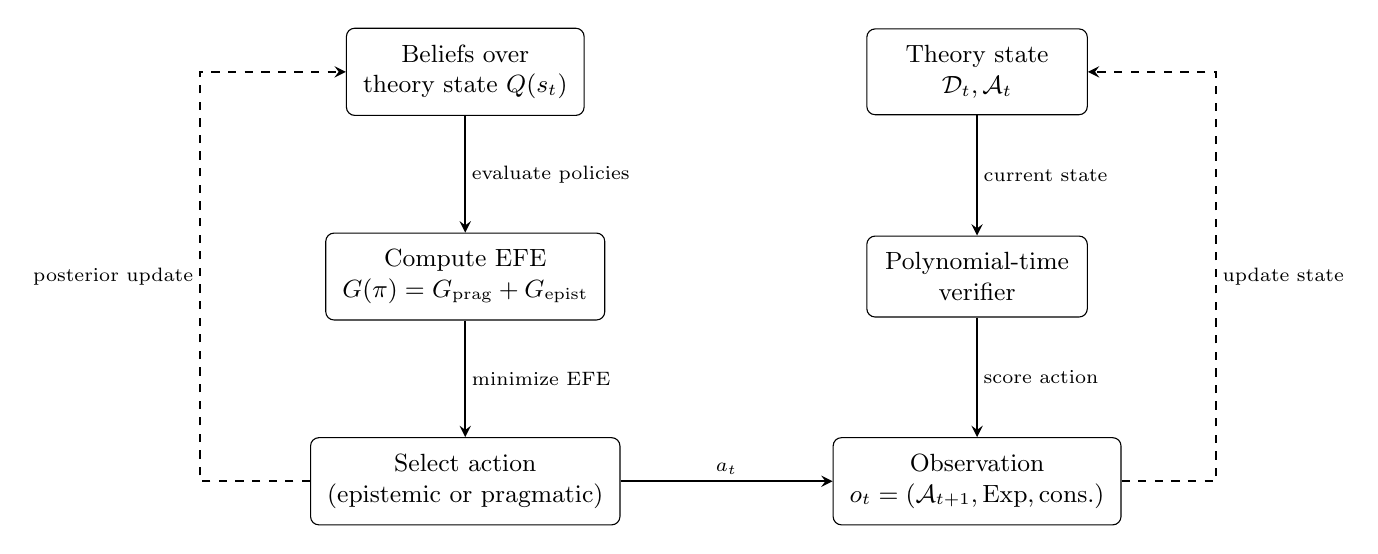
\begin{tikzpicture}[
    >=stealth,
    box/.style={
        draw, rounded corners=3pt,
        minimum height=1cm, minimum width=2.8cm,
        font=\small, inner sep=6pt,
        text centered, align=center
    },
    arr/.style={->, thick},
    lbl/.style={font=\scriptsize, fill=white, inner sep=2pt},
]

% Left column: Agent loop (x = 0)
\node[box] (beliefs) at (0, 0) {Beliefs over\\theory state $Q(s_t)$};
\node[box] (efe) at (0, -2.6) {Compute EFE\\$G(\pi) = G_{\mathrm{prag}} + G_{\mathrm{epist}}$};
\node[box] (action) at (0, -5.2) {Select action\\(epistemic or pragmatic)};

% Right column: Environment (x = 6.5)
\node[box] (theory) at (6.5, 0) {Theory state\\$\D_t, \mathcal{A}_t$};
\node[box] (verifier) at (6.5, -2.6) {Polynomial-time\\verifier};
\node[box] (obs) at (6.5, -5.2) {Observation\\$o_t = (\mathcal{A}_{t+1}, \Exp, \mathrm{cons.})$};

% Agent loop (left column, downward)
\draw[arr] (beliefs) -- node[lbl, right] {evaluate policies} (efe);
\draw[arr] (efe) -- node[lbl, right] {minimize EFE} (action);

% Action sent to observation (horizontal, bottom row)
\draw[arr] (action.east) -- node[lbl, above] {$a_t$} (obs.west);

% Theory feeds verifier (right column, downward)
\draw[arr] (theory) -- node[lbl, right] {current state} (verifier);

% Verifier produces observation (right column, downward)
\draw[arr] (verifier) -- node[lbl, right] {score action} (obs);

% Feedback: observation updates theory state (right side, going wide right then up)
\draw[arr, dashed] (obs.east) -- ++(1.2, 0) |- node[lbl, right, pos=0.25] {update state} (theory.east);

% Feedback: observation updates beliefs (left side, going wide left then up)
\draw[arr, dashed] (action.west) -- ++(-1.4, 0) |- node[lbl, left, pos=0.25] {posterior update} (beliefs.west);

\end{tikzpicture}
\end{center}

The loop operates as follows. The agent maintains beliefs $Q(s_t)$ over the current theory state. It evaluates candidate policies by computing EFE, decomposed into pragmatic value (will this action resolve anomalies?) and epistemic value (will this action reveal useful structure?). It selects the action minimizing EFE, which may be an epistemic probe (e.g., computing criticality of a rule) or a pragmatic revision (e.g., adding a defeater). The verifier scores the action and produces an observation. The agent updates its beliefs and repeats.

The critical difference from the GRPO workflow in Section~5: GRPO generates all candidates in parallel and scores them in one batch. Active Inference operates sequentially, using the result of each action to inform the next. This enables multi-step theory construction where early epistemic actions narrow the search space for later pragmatic actions.

\subsection{Neural-Guided Tree Search}

The preceding approaches either generate candidates in one shot (GRPO) or operate sequentially with analytically computed guidance (Active Inference minimizes EFE). A fourth approach, pioneered by AlphaGo~\cite{silver2016alphago} and refined through AlphaGo Zero~\cite{silver2017alphagozero}, AlphaZero~\cite{silver2018alphazero}, and MuZero~\cite{schrittwieser2020muzero}, introduces \emph{learned} policy and value functions that steer Monte-Carlo tree search through the state space. The resulting expert iteration loop---where search improves the networks and better networks improve the search---has achieved superhuman performance in every domain where an exact verifier is available, most recently in formal mathematical reasoning via AlphaProof~\cite{alphaproof2025}.

The structural analogy between board games and defeasible theory construction is precise. In Go, a position is a configuration of stones; in our setting, a position is a theory state $(\D_t, \mathcal{A}_t)$. In Go, a move places a stone; in our setting, an action proposes a rule, a defeater, or a superiority relation. In Go, the outcome is win or loss; in our setting, the outcome is the verifier's composite score. The polynomial-time verifier plays the role that the rules of Go play in AlphaZero: it defines a deterministic, model-independent transition function and terminal reward, which is exactly the structure that neural-guided tree search exploits.

\subsubsection{Policy and Value Networks}

Two networks are trained jointly on data generated by search:

\begin{itemize}[nosep]
    \item \textbf{Policy network} $p_\theta(a \mid s_t)$: given a theory state $s_t = (\D_t, \mathcal{A}_t)$, outputs a distribution over candidate theory modifications. This narrows the branching factor of the search tree, concentrating exploration on modifications that prior experience suggests are promising.
    \item \textbf{Value network} $v_\phi(s_t)$: given a theory state, predicts the expected terminal verifier score under continued optimal play. This truncates search depth: rather than rolling out every branch to termination, the value network provides a learned position evaluation at intermediate states.
\end{itemize}

In AlphaZero, a single network with two heads produces both outputs. The same architecture applies here: the input is a representation of the current theory state (the rule set, the anomaly set, the superiority relation), and the two heads predict the action distribution and the expected score respectively.

\subsubsection{MCTS over the Derivation Space}

Search proceeds as in AlphaZero. Each node in the search tree corresponds to a theory state. At each node, the algorithm selects the action maximizing an upper confidence bound:
\[
    a_t = \arg\max_a \Bigl( Q(s_t, a) + c_{\mathrm{puct}} \cdot p_\theta(a \mid s_t) \cdot \frac{\sqrt{\sum_b N(s_t, b)}}{1 + N(s_t, a)} \Bigr)
\]
where $Q(s_t, a)$ is the current action-value estimate, $N(s_t, a)$ is the visit count, and $c_{\mathrm{puct}}$ controls the exploration-exploitation tradeoff. The policy network prior $p_\theta(a \mid s_t)$ biases search toward promising modifications; the visit-count term ensures under-explored branches are not neglected.

When a leaf node $s_L$ is reached, the value network evaluates it: $v_\phi(s_L)$. If the leaf is terminal (all anomalies resolved or budget exhausted), the verifier provides the exact score. The value estimate is backed up through the tree, updating $Q$ values along the traversed path. After a fixed number of simulations, the algorithm selects the action with the highest visit count from the root.

The polynomial-time verifier provides an advantage that Go lacks: intermediate states can be \emph{exactly} evaluated (recompute $\mathcal{A}_t$, check conservativity) at polynomial cost. This means the value network can be supplemented or validated by the verifier at any node, not only at terminal states. The search can mix learned evaluation (fast, approximate) with verified evaluation (slower, exact), analogous to AlphaGo's mixing of value network evaluations with rollout outcomes.

\subsubsection{Expert Iteration}

The training loop follows AlphaZero's expert iteration:
\begin{enumerate}[nosep]
    \item \textbf{Self-play with search.} For each conflict $(r_A, r_B, q)$, run MCTS from the initial theory state $(\D, \mathcal{A})$. The search tree produces a policy target (the visit-count distribution at each visited node) and a value target (the terminal verifier score backed up to each visited node).
    \item \textbf{Network update.} Train $p_\theta$ to match the search policy (cross-entropy loss) and $v_\phi$ to predict the terminal score (mean squared error). The search policy is stronger than the raw network policy because it incorporates lookahead; training the network to match it is a form of policy improvement.
    \item \textbf{Iterate.} The improved network guides the next round of search, producing stronger policy and value targets. The loop converges when the network's raw predictions match the search-improved policy.
\end{enumerate}

This loop is self-reinforcing: better networks produce more focused search trees, and more focused search trees produce better training targets. AlphaZero demonstrated that this loop, starting from random initialization, converges to superhuman play in Go, chess, and shogi within hours of training. AlphaProof~\cite{alphaproof2025} demonstrated that the same loop, applied to formal theorem proving in Lean with the Lean kernel as verifier, solves International Mathematical Olympiad problems at silver-medal level.

\subsubsection{Relationship to the Training Pipeline}

The AlphaZero lineage suggests a correspondence with the three-phase pipeline of Section~5:

\begin{center}
\small
\begin{tabular}{@{}lll@{}}
\toprule
Pipeline Phase & AlphaGo (2016) & AlphaZero (2017+) \\
\midrule
Phase 1 (SFT) & SL policy from human games & Eliminated (tabula rasa) \\
Phase 2 (DPO) & RL policy via self-play & Subsumed by expert iteration \\
Phase 3 (RLVR) & Value network + MCTS & Unified: search \emph{is} the RL \\
\bottomrule
\end{tabular}
\end{center}

The original AlphaGo required all three phases. AlphaGo Zero and AlphaZero collapsed them: the expert iteration loop performs policy improvement (replacing DPO) and value learning (replacing separate reward modeling) simultaneously, bootstrapping from random initialization without human data (eliminating SFT). Whether the defeasible derivation space is structured enough for tabula rasa learning to bootstrap---or whether the SFT and DPO warm-start phases remain necessary---is an empirical question that depends on the density of valid defeaters in the search space relative to the branching factor.

\subsubsection{Neural-Guided Search vs. Active Inference}

Neural-guided tree search and Active Inference (Section~4.4.2) both operate sequentially over the theory construction MDP. They differ in how they guide the search:

\begin{center}
\small
\begin{tabular}{@{}lll@{}}
\toprule
Property & Neural-Guided Search & Active Inference \\
\midrule
Action evaluation & Learned ($p_\theta$, $v_\phi$) & Analytic (EFE decomposition) \\
Exploration mechanism & UCB with policy prior & Epistemic value term \\
Exploitation mechanism & Value network backup & Pragmatic value term \\
Belief state & Implicit (encoded in $v_\phi$) & Explicit ($Q(s_t)$ maintained) \\
Training signal & Expert iteration (search $\to$ network) & Not specified (framework, not algorithm) \\
Empirical validation & AlphaZero, AlphaProof & Limited to date \\
\bottomrule
\end{tabular}
\end{center}

The two approaches are not mutually exclusive. Active Inference's epistemic/pragmatic decomposition could inform the design of the policy network's action space (separating probing actions from revision actions), while the neural-guided search framework provides the concrete training algorithm that Active Inference lacks. A hybrid would use EFE-inspired action decomposition within an AlphaZero-style expert iteration loop.

\subsubsection{Connection to AlphaProof}

AlphaProof~\cite{alphaproof2025} instantiates precisely this architecture for formal mathematics. Its components map onto ours:

\begin{itemize}[nosep]
    \item \textbf{State}: a Lean proof state (goals, hypotheses, context) $\leftrightarrow$ a defeasible theory state $(\D_t, \mathcal{A}_t)$
    \item \textbf{Actions}: Lean tactics (apply, intro, rw, simp) $\leftrightarrow$ theory modifications (propose rule, propose defeater, assert superiority)
    \item \textbf{Verifier}: Lean's kernel (exact, sound, deterministic) $\leftrightarrow$ the polynomial-time defeasible logic engine
    \item \textbf{Search}: MCTS with AND-OR tree decomposition $\leftrightarrow$ MCTS over the derivation tree
    \item \textbf{Training}: expert iteration with test-time RL $\leftrightarrow$ expert iteration with self-play on conflicts
\end{itemize}

This correspondence is not incidental. Section~6 establishes an isomorphism between defeasible theories and formalized mathematical libraries, with Lean serving as the verifier in both settings. AlphaProof validates that neural-guided tree search with a formal verifier scales to competition-level mathematics. The proposal here extends the same paradigm to the broader class of defeasible conflicts---biomedical, ontological, and mathematical---that the DeFAb pipeline addresses.

DeepSearch~\cite{deepsearch2026} provides further evidence that this paradigm generalizes: it embeds MCTS directly into the RLVR training loop for LLM mathematical reasoning, demonstrating that tree-search-augmented training overcomes the performance plateaus that afflict standard GRPO.

\subsubsection{Two-Principle Search-Space Reduction}

The defining technical insight of AlphaGo~\cite{silver2016alphago} was the reduction of an intractable game-tree search of size $b^d$ along two principles: \emph{depth} is reduced by a learned position-evaluation function $v(s) \approx v^*(s)$ that truncates rollouts before they reach a terminal state; \emph{breadth} is reduced by a learned policy $p(a \mid s)$ that narrows the action set from all legal moves to a high-probability beam. Quantitatively, the principles must do real work: chess has $b \approx 35$ and $d \approx 80$, while Go has $b \approx 250$ and $d \approx 150$. Pure depth-first minimax was tractable for chess (Deep Blue) but intractable for Go.

The defeasible theory construction MDP exhibits an analogous structure but with markedly different magnitudes. The depth of construction is bounded above by $|\D|$ since each action adds one element to the theory, so for a starting theory of $\sim$200 rules the natural depth is comparable to chess. The branching factor, however, is the size of the defeater language $|\mathcal{L}_\D|$. For a theory with predicate signature $|\Sigma| = 50$, constant domain $|C| = 1{,}000$, and antecedent length bound $k = 3$, the count of well-formed defeaters is on the order of $\sum_{i=0}^{3} \binom{50 \cdot 1{,}000}{i} \cdot 2 \cdot 50 \cdot 1{,}000 \approx 10^{12}$, well beyond Go's branching factor by ten orders of magnitude. The asymmetry argues that the policy network's pruning role is \emph{more} critical for defeasible theory construction than for Go, and that the value network's depth-truncation role is \emph{less} critical (since rollouts terminate quickly). This shapes the engineering trade-off: aggressive policy regularization is essential, while value-network compute can be traded against verifier compute (Section~\ref{subsubsec:mixed-leaf}).

\subsubsection{Mixed Leaf Evaluation with the Exact Verifier}\label{subsubsec:mixed-leaf}

AlphaGo's APV-MCTS combines two leaf evaluators with a mixing parameter:
\[
    V(s_L) = (1 - \lambda) \, v_\theta(s_L) + \lambda \, z_L
\]
where $v_\theta$ is the value network and $z_L$ is the outcome of a fast rollout from $s_L$ to game termination. AlphaGo's ablation found $\lambda = 0.5$ optimal: value network and Monte Carlo rollout have complementary error profiles, and mixing them outperforms either alone~\cite{silver2016alphago}.

The defeasible setting offers a strict strengthening of this scheme. The polynomial-time verifier produces $z_L$ \emph{deterministically and exactly} on the partial theory $\D_L$ at the leaf, with no rollout noise:
\[
    z_L = \Score(\D_L, q) \quad \text{(exact, deterministic, polynomial-time)}.
\]
The naive prior is therefore $\lambda \to 1$: always trust the verifier. Two considerations recover an interior optimum. First, the verifier costs $O(|\D_L|^2 \cdot |F|)$, while $v_\theta$ is a single network forward pass with constant cost; under tight per-move time budgets (analogous to Go time controls), reserving the verifier for high-uncertainty nodes is rational. Second, the value network's prediction conditions on the entire trajectory by which the leaf was reached, encoding lookahead information that the local verifier call does not see. A practical recipe sets $\lambda = 1$ at terminal nodes (where the verifier output is exact and final) and $\lambda \in (0, 1)$ at non-terminal interior nodes (where $v_\theta$ amortizes the verifier compute), with the choice tuned on held-out search efficiency. AlphaGo's $\lambda = 0.5$ becomes a starting point, not an endpoint.

\subsubsection{The AlphaZero Loss for Defeasible Theories}

AlphaGo Zero~\cite{silver2017alphagozero} collapses the separate policy and value networks into a single dual-headed network $f_\theta(s) = (p_\theta(s), v_\theta(s))$, trained by minimizing the combined loss
\[
    \ell(\theta) = (z - v_\theta(s))^2 \;-\; \pi^\top \log p_\theta(s) \;+\; c \, \|\theta\|^2_2,
\]
where $z \in \{-1, +1\}$ is the self-play game outcome, $\pi$ is the MCTS visit-count distribution at the root ($\pi_a \propto N(s, a)^{1/\tau}$), and $c$ is an L2 regularization coefficient. The MSE term trains $v_\theta$ to predict the eventual outcome; the cross-entropy term trains $p_\theta$ to match the search-improved policy.

Adapting to defeasible theory construction, $z$ becomes the verifier-backed terminal score from a self-played conflict resolution game (Definition~2), normalized to $[-1, +1]$:
\[
    z = 2 \cdot \frac{\Score(d_{\mathrm{final}}, \D, q) - \min \Score}{\max \Score - \min \Score} - 1,
\]
and $s$ is the theory-state encoding $(\D_t, \mathcal{A}_t)$. The loss is otherwise identical. The empirical lesson from AlphaGo Zero's architecture ablation (Fig.~4 of \cite{silver2017alphagozero}) is striking: the dual-headed residual network outperforms separate policy and value networks by roughly 600 Elo, and the residual tower outperforms a non-residual convolutional tower by another 600 Elo. Combining policy and value into a shared trunk acts as regularization, forcing the network toward representations that support both tasks. We carry this prior into the recommended starting architecture: a 20-block residual or transformer trunk with a 256-dimensional hidden width, a policy head outputting a distribution over the typed defeater language $\mathcal{L}_\D$, and a value head outputting a scalar in $[-1, +1]$ via a $\tanh$ nonlinearity.

\subsubsection{Policy Iteration Framing of Expert Iteration}

The expert iteration loop described above can be made formally precise as classical approximate policy iteration~\cite{silver2017alphagozero,parr2022active}. Two operators alternate. \emph{Policy improvement}: MCTS, when run to convergence with the current network as prior and value, produces a search policy $\pi = \alpha_\theta(s)$ that is provably stronger than the raw network policy $p_\theta(s)$ because it incorporates lookahead. The proof is the standard policy-improvement theorem applied to the search-derived $Q$-values. \emph{Policy evaluation}: self-play games against the current best player produce trajectories $(s_t, \pi_t, z_t)$ whose terminal outcomes $z_t$ are samples of the value function under the improved policy. The training step projects $(\pi, z)$ back into the network's function space by gradient descent on the AlphaZero loss above.

The AlphaGo Zero \emph{evaluator} provides a concrete acceptance gate that disciplines this loop: a new network checkpoint replaces the current best player only if it wins more than 55\% of evaluation games against it, screening out gradient-descent noise from genuine policy improvement. We adopt the same gate. In our setting, an ``evaluation game'' is a fresh defeasible conflict drawn from a held-out partition; the new checkpoint serves as the policy and value network for both sides; the verifier scores the resulting defeaters; the win rate is computed as the fraction of conflicts where the new checkpoint produces a defeater that strictly dominates (higher composite score) the one produced by the current best. This replaces the vague ``iterate'' instruction with a measurable criterion.

\subsubsection{Diversity vs.\ Sharpness in the Policy Prior}

A subtle but important finding in AlphaGo~\cite{silver2016alphago} is that the supervised-learning policy network $p_\sigma$ (trained on human expert games) outperformed the reinforcement-learning policy network $p_\rho$ (trained by self-play policy gradient) when used as the MCTS prior, even though $p_\rho$ won 80\% of head-to-head games against $p_\sigma$ when used directly. Silver et al.\ attribute the reversal to a diversity-versus-sharpness trade-off: humans select among many plausible moves, so $p_\sigma$ produces a broad beam that gives MCTS multiple candidate branches to explore; $p_\rho$ converges toward a single optimal move and starves the search of branches.

The same trade-off is visible in our pipeline (Section~5). The SFT-trained model (Phase~1) is broad: trained on diverse gold hypotheses, it spreads probability mass across many plausible defeaters per conflict. The DPO-tuned model (Phase~2) is sharper: trained on preference pairs, it concentrates probability on the highest-scoring defeater observed in training. The GRPO-tuned model (Phase~3) is sharpest. The AlphaGo lesson predicts that the SFT model gives the better MCTS prior despite scoring lower in direct evaluation, because conflicts in the Lakatos-correspondence sense (Proposition~6) typically admit multiple valid resolutions at varying conservativity levels, and the search needs to consider all of them. A concrete experimental design: hold the search algorithm and value head fixed, vary only the policy prior across $\{p_{\mathrm{SFT}}, p_{\mathrm{DPO}}, p_{\mathrm{GRPO}}\}$, and report MCTS-derived composite-score as a function of search budget.

\subsubsection{MCTS Engineering: Virtual Loss, Dirichlet Noise, Temperature, Resignation}

Four implementation details from AlphaGo and AlphaGo Zero transfer directly to defeasible MCTS. They are not optional refinements; without them the training loop fails to converge or wastes compute on hopeless paths.

\textit{Virtual loss.} When multiple search threads run in parallel, they must be discouraged from collapsing onto the same path. AlphaGo's solution is to apply a virtual loss $n_{\mathrm{vl}} = 3$ at each in-tree step of an in-flight simulation: the path appears as if it has lost $n_{\mathrm{vl}}$ games, depressing its UCB score and steering other threads elsewhere. The virtual loss is undone when the simulation completes. In the defeasible setting, this prevents redundant verifier calls on the same partial theory, which matters because verifier calls are CPU-expensive.

\textit{Dirichlet noise at the root.} To ensure that self-play exploration covers low-prior defeaters that the network would otherwise never sample, AlphaGo Zero adds Dirichlet noise to the root prior: $P(s_0, a) = (1 - \epsilon) p_a + \epsilon \eta_a$ with $\eta \sim \mathrm{Dir}(0.03)$ and $\epsilon = 0.25$. The concentration parameter 0.03 is chosen so that the Dirichlet sample is sparse, briefly elevating a small subset of low-prior actions per conflict. The same scheme applies to defeasible self-play: without root noise, the network will not generate training signal for defeaters outside its current support.

\textit{Temperature schedule.} For the first 30 moves of an AlphaGo Zero self-play game, the visit-count-derived play distribution uses temperature $\tau = 1$ (sample proportionally to visit count); thereafter $\tau \to 0$ (deterministic argmax). This interleaves diverse exploration in the opening with sharp commitment in the endgame. In defeasible self-play, the analog is to use $\tau = 1$ for the first $k$ defeater proposals in a conflict and $\tau \to 0$ thereafter, with $k$ tuned to the typical conflict-resolution depth.

\textit{Resignation threshold.} Many self-play games are decided long before termination; continuing them wastes compute. AlphaGo Zero resigns when the root value $Q(s_0)$ drops below a threshold $v_{\mathrm{resign}}$, calibrated to keep the rate of false positives (games that could have been won) below 5\% by disabling resignation in 10\% of games and measuring. The same threshold logic applies to defeasible conflicts: skip a conflict when the verifier's composite-score estimate at the root drops below $v_{\mathrm{resign}}$, recovering compute for harder conflicts.

\subsubsection{Asynchronous APV-MCTS Architecture for Defeasible Search}

AlphaGo's distributed search architecture~\cite{silver2016alphago} maps directly onto the defeasible setting. A master node holds the search tree and executes the in-tree phase of each simulation. Remote CPU workers execute the rollout phase: in AlphaGo this meant playing fast rollouts to game termination; in our setting it means running the polynomial-time defeasible engine on the extended theory $\D \cup \{d\}$ to produce the exact $z_L$. Remote GPU workers execute the network forward passes producing $(p_\theta, v_\theta)$ at expanded leaves. The master communicates leaf positions to the workers, receives evaluations asynchronously, and backs them up through the search tree.

The architecture suits the defeasible compute profile. The defeasible engine is CPU-bound and embarrassingly parallel across distinct partial theories; the dual-headed network is GPU-bound and benefits from batched evaluation. AlphaGo's scalability table (Extended Data Table~8 of \cite{silver2016alphago}) reports near-linear scaling from 1 to 40 search threads on 8 GPUs, and from 8 GPUs to 280 GPUs in the distributed setting. The same scaling regime is available on CURC Alpine, where each compute node provides multiple A100 GPUs and 64+ CPU cores; the verifier rollout pool can saturate the CPU cores while the network worker pool keeps the GPUs fed.

\subsubsection{Domain Knowledge for Defeasible AlphaZero}

AlphaGo Zero explicitly enumerates the domain knowledge it uses, to make precise that everything else is learned~\cite{silver2017alphagozero}. The list comprises (1) game rules and termination, (2) Tromp--Taylor scoring, (3) the $19 \times 19$ board structure (matched by the convolutional architecture), and (4) dihedral and color-transposition invariances. The same enumeration discipline is appropriate for a Defeasible AlphaZero specification:

\begin{enumerate}[nosep]
    \item \textbf{Defeasible derivation rules.} The Antoniou--Billington--Governatori conditions for $+\partial q$ are provided as the transition function: given $(\D_t, a_t)$, the verifier deterministically produces $\D_{t+1} = \D_t \cup \{a_t\}$ and the updated anomaly set $\mathcal{A}_{t+1}$.
    \item \textbf{Verifier scoring function.} The scoring function $\Score(d, \D, q)$ is provided as the terminal reward; the network does not approximate it.
    \item \textbf{Theory state encoding.} The rule set, anomaly set, and superiority relation are passed to the network as a permutation-invariant graph (each rule a node, antecedent--consequent and superiority edges) or as a tokenized text representation under a fixed schema. The architecture is matched to the encoding (graph neural network or transformer over tokens).
    \item \textbf{Predicate-renaming invariance.} The natural analog of AlphaGo Zero's dihedral symmetries is that a defeasible theory under a bijective relabeling of predicate symbols has the same proof structure. This invariance can be exploited by data augmentation (random renaming during training) and by symmetry ensembling at inference (averaging network outputs over renaming samples), exactly mirroring AlphaGo Zero's symmetry handling.
\end{enumerate}

No domain-specific heuristics, no handcrafted defeater patterns, no priority biases beyond the verifier itself. Anything beyond items 1--4 must be learned from self-play.

\subsubsection{Tabula Rasa Feasibility: Quantitative Grounding}

AlphaGo Zero's most striking empirical result is that random initialization is sufficient: starting from uniform-random weights, the system surpasses AlphaGo Lee within 36 hours and AlphaGo Master within 40 days~\cite{silver2017alphagozero}. The result was unanticipated; prior work had assumed that supervised warm-start from human games was essential.

Whether the same result transfers to defeasible theory construction depends on the relationship between the policy network's effective branching factor (after pruning the $\sim 10^{12}$-element defeater language $\mathcal{L}_\D$) and the density of valid defeaters in that space. In Go, the random-initialization policy still concentrates probability on \emph{some} legal moves, and self-play exploration with Dirichlet noise eventually finds informative gradients. In defeasible construction, a uniform prior over $\mathcal{L}_\D$ assigns vanishing probability to any specific valid defeater, and the gradient signal from random rollouts may be too sparse to bootstrap. The branching-factor disparity (Go $b \approx 250$, defeasible $b \sim 10^{12}$) suggests that aggressive prior shaping via SFT warm-start (Phase~1 of Section~5) likely remains rational engineering even if tabula-rasa is theoretically feasible. A concrete empirical test: ablate Phase~1 on a small Tier-0-derived training run, hold Phase~2 and Phase~3 fixed, and compare self-play composite-score trajectories at 24h, 48h, and 72h. If the random-init trajectory catches up, tabula-rasa is feasible; if it stalls, the SFT prior is doing irreplaceable work.

\subsubsection{Dual-Head vs.\ Separate Networks: Architecture Ablation Plan}

AlphaGo Zero's Fig.~4 reports a four-cell ablation that decomposes its architectural advance over AlphaGo Lee into two roughly equal contributions: residual versus convolutional towers ($\sim$600 Elo), and dual-headed versus separate policy and value networks ($\sim$600 Elo). The combination (\emph{dual-res}) wins by $\sim$1{,}200 Elo over the combination used in AlphaGo Lee (\emph{sep-conv}).

The ablation should be replicated for Defeasible AlphaZero once the pipeline is operational. A 20-block trunk (residual CNN over a graph encoding, or transformer over a tokenized encoding) with 256-dimensional hidden width matches the AlphaGo Zero starting configuration, and the four-cell ablation (dual-res, dual-conv, sep-res, sep-conv) is mechanical to implement once the data pipeline is in place. The expected qualitative result is the AlphaGo Zero ordering, but the magnitudes will differ: the regularization gain from a shared trunk is largest when the policy and value heads benefit from \emph{different} representations of the same input, which holds for Go (move-shape information vs.\ winning-territory information) and is plausible but not certain for defeasible reasoning. The ablation is therefore both expected and informative.

\subsubsection{DeFAb-Hard as the Proper Evaluation Surface}

A capability-establishing experiment for the Defeasible AlphaZero pipeline must be run on instances that current frontier models reproducibly fail. The existing 35-instance Tier~0 Level~3 set does not satisfy this property: reasoning-optimized models under chain-of-thought scaffolding (DeepSeek-R1 92.9\%, GPT-5.2-chat 87.1\%) approach a ceiling that compresses any improvement signal from neural-guided search to within the noise of the Wilson 95\% confidence interval ($\pm 15$--$17$~pp at $n = 35$). Running the AlphaZero loop against an already-saturated benchmark would produce no measurable training signal regardless of whether the underlying capability gain is real.

The companion paper introduces DeFAb-Hard, a structurally pre-registered Level~3 subset stratified along four orthogonal axes: high predicate novelty ($\Nov(r^*, \Dm) \geq 0.5$, target 1{,}000 instances), scaled theory size and support depth ($|\D| \in \{50, 100, 200\}$, depth $\geq 5$, $\geq 3$ competing defaults, target 300 instances), multi-anomaly conservativity ($k \geq 3$ unrelated anomalies, target 100 instances), and the pending 409-instance synthetic contamination evaluation. The pre-registered prediction is that the strongest model under the strongest prompting strategy drops by at least 30 percentage points on the four-axis intersection cell relative to the easy 35-instance baseline. The intersection cell is the structurally hardest region of the benchmark: an instance there demands a high-novelty defeater operating at depth $\geq 5$ in a 200-rule theory while preserving the derivability of three independent unrelated anomalies. This is also the region where the defeater language $|\La_\D| \sim 10^{12}$ argument of the two-principle subsubsection has bite: aggressive policy pruning is required, the value network must amortize the verifier across non-trivial branching, and the conservativity check is no longer a default-pass.

The Defeasible AlphaZero pipeline should therefore be evaluated on DeFAb-Hard as its primary benchmark, with the easy 35-instance set retained as a calibration anchor for cross-study comparability. The expert iteration loop is allowed to overfit to the easy set; what matters is the trajectory on the intersection cell. If neural-guided tree search closes a non-trivial fraction of the H\textsubscript{HARD} gap (e.g., from a baseline 30~pp drop to a 10~pp drop) while the SFT/DPO/GRPO pipeline alone does not, the AlphaGo-lineage recipe earns its place in the defeasible setting empirically rather than by analogy. The ablation table reports H\textsubscript{HARD} accuracy under \{base, SFT, DPO, GRPO, neural-guided MCTS\} for each of the four panel models, with the AlphaZero column populated only after expert iteration converges by the AGZ-style $>$55\% acceptance gate.

\section{Unified Training Pipeline}

\begin{center}
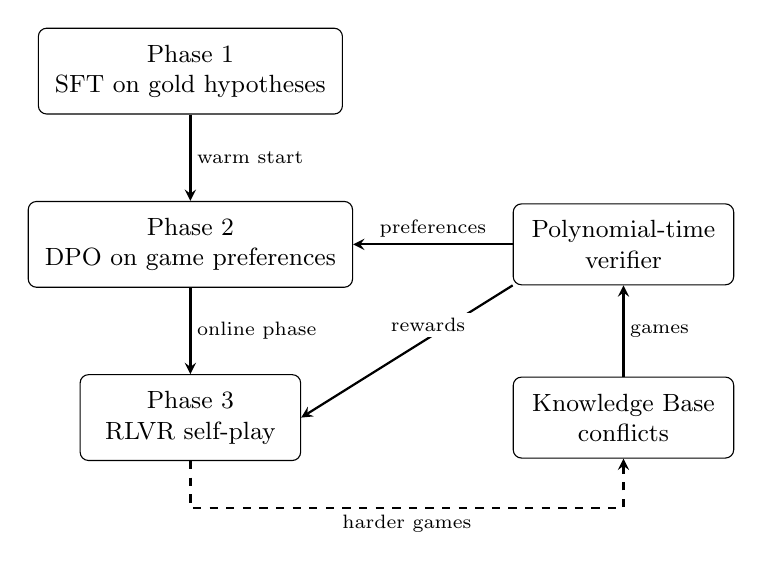
\begin{tikzpicture}[
    >=stealth,
    box/.style={
        draw, rounded corners=3pt,
        minimum height=1cm, minimum width=2.8cm,
        font=\small, inner sep=6pt,
        text centered, align=center
    },
    arr/.style={->, thick},
    lbl/.style={font=\scriptsize, fill=white, inner sep=2pt},
]

% Layout: two columns, left = pipeline (vertical), right = infrastructure (vertical)
% Left column: three training phases stacked vertically
\node[box] (sft) at (0, 0) {Phase 1\\SFT on gold hypotheses};
\node[box] (dpo) at (0, -2.2) {Phase 2\\DPO on game preferences};
\node[box] (rlvr) at (0, -4.4) {Phase 3\\RLVR self-play};

% Right column: verifier and KB
\node[box] (verifier) at (5.5, -2.2) {Polynomial-time\\verifier};
\node[box] (kb) at (5.5, -4.4) {Knowledge Base\\conflicts};

% Pipeline flow (left column, downward)
\draw[arr] (sft) -- node[lbl, right] {warm start} (dpo);
\draw[arr] (dpo) -- node[lbl, right] {online phase} (rlvr);

% Verifier provides preferences to DPO (horizontal)
\draw[arr] (verifier.west) -- node[lbl, above] {preferences} (dpo.east);

% Verifier provides rewards to RLVR (horizontal)
\draw[arr] (verifier.south west) -- node[lbl, above, pos=0.4] {rewards} (rlvr.east);

% KB feeds games into verifier (vertical)
\draw[arr] (kb) -- node[lbl, right] {games} (verifier);

% Feedback loop: RLVR generates harder games back to KB
\draw[arr, dashed] (rlvr.south) -- ++(0, -0.6) -|
    node[lbl, below, pos=0.25] {harder games} (kb.south);

\end{tikzpicture}
\end{center}

Phase 1 (SFT): train on gold hypotheses from existing DeFAb instances. Establishes baseline format compliance and grounding capability.

Phase 2 (DPO): train on game-generated preferences. MCTS pre-computes conflict resolutions offline. The margin-weighted loss internalizes the ordinal structure of conflict resolution quality.

Phase 3 (RLVR): online self-play with GRPO. The model generates defeaters in real time. The verifier provides exact rewards. The feedback loop between model improvement and game difficulty creates an automatic curriculum.

The verifier is the fixed point. It never degrades, never approximates, never drifts. Every training signal, whether preference or reward, is mathematically verified.

\section{Extension to Formalized Mathematics}

The Lakatosian foundation makes the extension to formalized mathematics natural. The isomorphism between DeFAb theories and mathematical proof libraries is precise:

\begin{itemize}[nosep]
    \item \textbf{Strict rules} from proven theorems. \texttt{theorem foo (h1: C1) (h2: C2) : P} becomes $r_s\colon C_1, C_2 \strictto P$, validated by Lean's kernel.
    \item \textbf{Defeasible rules} from weakened theorems. Dropping condition $C_2$ yields $r_d\colon C_1 \defto P$, a conjecture that is usually true but admits exceptions when $C_1 \wedge \neg C_2$ holds.
    \item \textbf{Defeaters} from counterexamples. An instance $a$ with $C_1(a) \wedge \neg C_2(a) \wedge \neg P(a)$ is a falsifier that defeats $r_d$.
    \item \textbf{Conservativity} from the full theorem. The defeater must block $P$ only in the exception region $(\neg C_2)$, preserving every instance where all original conditions hold.
\end{itemize}

The defeasible conflict game applies directly. Two conflicting conjectures (weakened theorems with overlapping but incompatible domains) are resolved by constructing counterexamples that determine which conjecture should yield. Lean serves as the verifier: exact, sound, complete, and requiring no approximation.

\textit{Example.} Euler's formula $V - E + F = 2$. The defeasible rule: this holds for all polyhedra. The defeater: polyhedra with genus $> 0$ (a torus has $V - E + F = 0$). At Level~3, the model must construct the genus-based exception without breaking the formula for convex polyhedra. Lakatos devoted an entire book to the dialectical history of exactly this conjecture.

\textit{Example.} ``Convergent sequences of continuous functions have continuous limits.'' The defeater: pointwise (not uniform) convergence may yield discontinuous limits. The refined conjecture is a strict rule in Mathlib (\texttt{TendstoUniformly.continuous}). The game: Player~A argues for the pointwise convergence conjecture; Player~B constructs the counterexample. The verifier (Lean) confirms the counterexample and checks that the refinement to uniform convergence preserves all valid instances.

\section{Open Questions}

\begin{enumerate}
    \item \textbf{Is RLVR Necessary?} Learned preferences via the defeasible games may be adequate and RLVR may not provide tangible benefit. This must be experimentally verified via ablation.
    \item \textbf{How is novelty computed?} We indicate earlier that novelty can be computed, but provide no explicit formulation. There are several clear possibilities which can be tried (Information-theoretic surprisal, topological novelty on the dependency graph), and we must verify a novelty modifier is even required at all. Parsimony or conservativity alone may be sufficient for exploring the decision space.
    \item \textbf{Conflict enumeration at scale.} How many distinct conflicts exist in UMLS, SNOMED, GO? Is the number tractable for exhaustive game generation, or do we need sampling strategies?
    \item \textbf{Game balance.} Are most conflicts ``one-sided'' (one resolution is clearly superior)? If so, the preference signal may be redundant. How many conflicts admit competitive resolutions where MCTS search depth matters?
    \item \textbf{Self-play stability.} Does the self-play dynamic converge, or does it oscillate? The verifier prevents reward hacking, but the model could cycle between favoring Rule A and Rule B without settling.
    \item \textbf{Process vs.\ outcome reward.} Does step-level reward from derivation decomposition actually improve credit assignment, or does the additional complexity of step scoring introduce noise?
    \item \textbf{Transfer to open-ended reasoning.} Models trained on KB-derived conflicts learn to resolve structured disagreements. Does this transfer to open-ended clinical reasoning where the theory is implicit rather than explicit?
    \item \textbf{Connection to drug discovery.} In the biomedical setting, a conflict between ``Drug X treats Condition Y'' and ``Drug X is contraindicated for Comorbidity Z'' is a clinical decision. Can defeasible self-play produce models that reason about pharmacogenomic exceptions without explicit pharmacogenomic training data?
    \item \textbf{Lakatos strategies as reward shaping.} Can the three Lakatosian refinement strategies (monster-barring, exception-barring, lemma-incorporation) be formalized as distinct reward components? If so, the training signal could distinguish \emph{how} the model refines a conjecture, not just whether the refinement is conservative.
    \item \textbf{Mathematics as the cleanest testbed.} Lean provides an exact verifier with no approximation. If the game-based fine-tuning framework works on DeFAb-Math (where verification is perfect), does the approach transfer to biomedical domains (where verification is polynomial-time but operates over noisier knowledge bases)?
    \item \textbf{Popper's asymmetry.} Popper observed that falsification is logically stronger than confirmation: a single counterexample refutes a universal claim, but no number of confirmations can prove one. Does this asymmetry manifest in the game dynamics? Is the opponent (falsifier) systematically advantaged over the proponent (conjecture defender)?
    \item \textbf{Epistemic vs.\ pragmatic sample efficiency.} Does the Active Inference formulation (Section~4.4) improve sample efficiency over GRPO by explicitly separating exploration from exploitation? The hypothesis: epistemic actions (probing theory structure) narrow the search space for subsequent pragmatic actions (constructing defeaters), reducing the number of rollouts needed to find valid resolutions.
    \item \textbf{Epistemic foraging for latent defeaters.} Can Active Inference discover defeaters that one-shot GRPO generation misses? If the theory has deep dependency chains, epistemic actions that trace support sets may reveal distant vulnerability points invisible to single-step generation.
    \item \textbf{Lakatos as Active Inference trajectory.} Is the Lakatosian conjecture-counterexample-refinement cycle an optimal Active Inference policy? The counterexample search is an epistemic phase (maximizing information gain about where the conjecture fails), and the refinement is a pragmatic phase (resolving the anomaly conservatively). If Active Inference naturally recovers this two-phase structure, it provides a normative justification for the Lakatosian methodology.
    \item \textbf{Falsification as epistemic action.} Popperian falsification can be formalized as selecting the action with maximal epistemic value: the observation that most discriminates between competing theories. Does Active Inference's epistemic term naturally produce falsification-seeking behavior without explicit reward shaping?
    \item \textbf{Active Inference vs.\ curriculum scheduling.} Does the epistemic/pragmatic balance in Active Inference replace the need for manual curriculum scheduling (Section~5)? If epistemic value naturally decreases as the agent learns the theory's structure, the transition from exploration to exploitation is automatic.
    \item \textbf{Tabula rasa feasibility.} AlphaGo Zero and AlphaZero demonstrated that the SL warm-start is unnecessary in Go, chess, and shogi---self-play from random initialization suffices. Does the defeasible derivation space admit the same? The density of valid defeaters relative to the branching factor determines whether random exploration can bootstrap. If the space is too sparse, the SFT and DPO phases may be prerequisites rather than accelerants.
    \item \textbf{Branching factor of the derivation space.} In Go, the branching factor is approximately 250; in chess, approximately 35. What is the effective branching factor of the defeasible theory construction space? Given a theory $\D$ with predicate signature $\Sigma$ and constant domain $C$, the naive branching factor is $|\mathcal{L}_\D|$ (the size of the defeater language), but the policy network's role is to reduce this to a tractable effective branching factor. How aggressive must the policy network's pruning be to make search feasible?
    \item \textbf{Learned dynamics as verifier proxy.} The polynomial-time verifier is exact but not free. For large knowledge bases, MuZero's insight applies: a learned dynamics model could predict verifier outputs (anomaly counts, conservativity status) without running the full engine. The learned model would serve as a fast proxy during search, with the exact verifier validating only terminal or high-uncertainty states. Under what conditions does the approximation error remain acceptable?
    \item \textbf{Mixed-evaluation tradeoff under exact verification.} AlphaGo's $\lambda = 0.5$ optimal mixing of value-network and Monte Carlo rollout reflects two stochastic estimators with complementary error profiles. With our deterministic exact $z_L = \Score(\D_L, q)$, the naive prior is $\lambda \to 1$ (always trust the verifier). Does an interior optimum survive once compute cost is accounted for? The cost model $\mathrm{cost}(z_L) = O(|\D_L|^2 \cdot |F|)$ versus $\mathrm{cost}(v_\theta) = O(1)$ favors $\lambda < 1$ at deep interior nodes. Empirical question: at what theory size does $v_\theta$-only evaluation outperform exact-verifier-only evaluation under fixed wall-clock budgets?
    \item \textbf{Tabula-rasa transfer between knowledge bases.} AlphaZero retrains from scratch for chess, Go, and shogi, treating each game as an independent training run. Defeasible knowledge bases share the defeasible-theory schema, so a Defeasible AlphaZero trained tabula-rasa on biology conflicts could in principle transfer to legal or biomedical conflicts via predicate-renaming-invariant features (Section on domain knowledge). Does this transfer hold empirically? Test by training random-init on biology-only conflicts, evaluating root-value calibration and search-policy quality on legal and materials conflicts at fixed compute budgets, and comparing against networks trained tabula-rasa on each target domain individually.
    \item \textbf{Does AlphaZero-style training close the DeFAb-Hard gap?} The pre-registered DeFAb-Hard prediction is that the strongest base model under the strongest prompting strategy drops by at least 30~pp on the four-axis intersection cell relative to the easy 35-instance baseline. The capability question for the AlphaZero-style pipeline is whether expert iteration with neural-guided MCTS and verifier-backed reward closes a non-trivial fraction of that gap. The ablation factors are \{base, SFT, DPO, GRPO, neural-guided MCTS\} on identical instances. A positive result on the H\textsubscript{HARD} intersection cell---closing, say, $\geq 15$ of the predicted 30~pp gap---would constitute the first empirical demonstration that AlphaZero-style search-and-network co-training transfers from games and formal mathematics to defeasible reasoning over real-world knowledge bases. A null result would indicate that the AlphaGo-lineage recipe does not transfer to this setting and would motivate a search for what is structurally different about defeasible theory construction.
    \item \textbf{Difficulty-vs-search-budget Pareto front.} For each cell of the DeFAb-Hard subset (H1 high-novelty, H2 scaled-depth, H3 multi-anomaly, H1$\cap$H2$\cap$H3 intersection), how does AlphaZero-style accuracy scale as a function of MCTS simulation budget per instance? The mixed-leaf evaluation argument predicts that the value-network share of total compute matters most when the verifier is expensive (large $|\D|$, deep support); the policy-network share matters most when the branching factor is large (high novelty). Mapping the Pareto front---accuracy as a function of (search budget, value-network compute share, policy-network compute share) per axis---tests these predictions and identifies the compute regime where AlphaZero-style search dominates pure GRPO and the regime where the two are equivalent. The result also informs deployment: where on the Pareto front does each cell saturate?
\end{enumerate}

\section{Formal Justification (WIP)}
 
The two-player structure of the conflict resolution game is not a modeling choice. It is forced by the proof theory of defeasible logic. This section makes the argument precise and establishes the formal properties that the training pipeline depends on: binarity, zero-sumness, finiteness, and determinacy.
 
\subsection{From Derivation Conditions to Games}
 
We begin with the standard derivation condition for defeasible provability. In the formulation of Antoniou, Billington, and Governatori~\cite{antoniou2001representation}, the condition $+\partial q$ holds in theory $\D$ if and only if:
 
\begin{enumerate}[nosep]
    \item There exists a rule $r \in R[q]$ such that every antecedent of $r$ is provable, and
    \item For every rule $s \in R[\comp{q}]$ whose antecedents are all provable, there exists a rule $t \in R[q]$ whose antecedents are all provable and $t > s$.
\end{enumerate}
 
The quantifier structure is $\exists \forall \exists$. This alternation defines a two-player evaluation game in the standard sense of logic and model theory. Let the \emph{proponent} control the existential quantifiers and the \emph{opponent} control the universal quantifier. The proponent selects a supporting rule $r$, the opponent selects an attacking rule $s$, and the proponent must counter with a superior rule $t$. A derivation succeeds if and only if the proponent has a winning strategy in this game. This connection between alternating quantifiers and two-player games is not metaphorical; it is the content of the game-theoretic semantics of Hintikka~\cite{hintikka1996principles} applied to the metalanguage of the derivation conditions.
 
\begin{proposition}[Binarity of Defeasible Conflict]\label{prop:binarity}
Let $\D$ be a defeasible theory and let $q$ be a literal. Under classical complementation, every conflict over $q$ in $\D$ partitions the relevant rules into exactly two sets: $R[q]$ and $R[\comp{q}]$. No rule bears on both sides, and no third position exists.
\end{proposition}
 
\begin{proof}
By the definition of a defeasible theory, every rule $r$ has a unique consequent $c(r)$. For a conflict over literal $q$, a rule is relevant if and only if $c(r) = q$ or $c(r) = \comp{q}$. Classical complementation is an involution ($\comp{\comp{q}} = q$), so $c(r) \in \{q, \comp{q}\}$ is an exhaustive and mutually exclusive partition of the relevant rules.
\end{proof}
 
\begin{remark}
Binarity is a consequence of classical negation, not of any domain assumption. A logic with three-valued complementation (e.g., where $q$, $\comp{q}$, and $\bot$ are distinct) could induce three-player conflicts. The restriction to two players is precisely the restriction to classical defeasible logic.
\end{remark}
 
\subsection{From Proof Games to Theory Construction Games}
 
The standard dialogical game operates over a fixed theory: given $\D$, does $+\partial q$ hold? Both the proponent and the opponent select from rules already present in $\D$. Our conflict resolution game (Definition~2) differs in a precise way: the theory is not fixed, and the players construct extensions to it.
 
\begin{definition}[Theory Construction Game]
Let $(r_A, r_B, q)$ be a defeasible conflict in $\D$. The theory construction game $\Gamma(\D, r_A, r_B, q)$ is a simultaneous-move game defined by:
\begin{enumerate}[nosep]
    \item \textbf{Strategy sets.} Player~A's strategy set is $S_A = \{d \in \mathcal{L}_\D \mid \D \cup \{d\} \vdash_\partial q \text{ and } \D \cup \{d\} \not\vdash_\partial \comp{q}\}$. Player~B's strategy set $S_B$ is defined symmetrically. Here $\mathcal{L}_\D$ is the defeater language over $\D$ (defined below).
    \item \textbf{Payoff.} The payoff to Player~A is $u_A(d_A, d_B) = \Score(d_A, \D, q) - \Score(d_B, \D, \comp{q})$, with $u_B = -u_A$.
\end{enumerate}
\end{definition}
 
Two properties of this game require proof: that it is zero-sum, and that it is finite (and therefore determined).
 
\begin{proposition}[Zero-Sum Structure]\label{prop:zerosum}
The theory construction game $\Gamma(\D, r_A, r_B, q)$ is zero-sum.
\end{proposition}
 
\begin{proof}
By construction, $u_B = -u_A$. It remains to show this is not merely a convention but reflects a logical constraint: no theory extension can simultaneously resolve the conflict in favor of both $q$ and $\comp{q}$.
 
Suppose for contradiction that there exists an extension $\D' \supseteq \D$ such that $\D' \vdash_\partial q$ and $\D' \vdash_\partial \comp{q}$ and the conflict $(r_A, r_B)$ is resolved. By the resolution condition (Definition~2), resolution in favor of $q$ requires $\D' \not\vdash_\partial \comp{q}$, and resolution in favor of $\comp{q}$ requires $\D' \not\vdash_\partial q$. Both conditions cannot hold simultaneously. Hence any resolution must favor exactly one side, and the gain of one player is the loss of the other.
\end{proof}
 
\subsection{Finiteness and Determinacy}
 
The standard dialogical game over a fixed theory is finite because defeasible proof trees are well-founded: they bottom out at facts and strict rules. The theory construction game introduces a new concern, since the players are not selecting from a fixed rule set but constructing new rules. The strategy space could in principle be infinite. The following definition and proposition establish that it is not.
 
\begin{definition}[Defeater Language]\label{def:defeater_lang}
Given a defeasible theory $\D$ with predicate signature $\Sigma$ and constant domain $C$, the defeater language $\mathcal{L}_\D$ is the set of all syntactically well-formed defeaters whose predicates are drawn from $\Sigma$, whose constants are drawn from $C$, and whose rule length (number of antecedents) is bounded by $k = \max_{r \in \D} |A(r)|$, the maximum antecedent length of any rule in $\D$.
\end{definition}
 
\begin{proposition}[Finiteness of Strategy Sets]\label{prop:finiteness}
If $\Sigma$ and $C$ are finite, then $\mathcal{L}_\D$ is finite, and therefore $S_A$ and $S_B$ are finite.
\end{proposition}
 
\begin{proof}
A defeater $d$ is specified by: a set of antecedents (a subset of the Herbrand base $\mathrm{HB}(\Sigma, C)$, bounded in size by $k$), a consequent (an element of $\mathrm{HB}(\Sigma, C)$ or its complement), and a target rule in $\D$. Since $\mathrm{HB}(\Sigma, C)$ is finite when $\Sigma$ and $C$ are finite, the number of possible antecedent sets of size at most $k$ is $\sum_{i=0}^{k} \binom{|\mathrm{HB}(\Sigma, C)|}{i}$, which is finite. The number of consequents is $2|\mathrm{HB}(\Sigma, C)|$, and the number of target rules is $|\D|$. The product is finite.
\end{proof}
 
\begin{remark}
The bound $k$ is a modeling choice, not a logical necessity. Without it, the strategy space remains finite (since $\Sigma$ and $C$ are finite, the Herbrand base is finite, and the powerset of a finite set is finite), but the bound ensures the strategy space is computationally manageable. In practice, defeaters in biomedical and mathematical theories rarely exceed the antecedent complexity of the rules they target, so the bound is not restrictive.
\end{remark}
 
\begin{proposition}[Determinacy]\label{prop:determinacy}
The theory construction game $\Gamma(\D, r_A, r_B, q)$ is determined: it has a value $v^*$ such that
\[
    v^* = \max_{d_A \in S_A} \min_{d_B \in S_B} u_A(d_A, d_B) = \min_{d_B \in S_B} \max_{d_A \in S_A} u_A(d_A, d_B).
\]
\end{proposition}
 
\begin{proof}
The game is finite (Proposition~\ref{prop:finiteness}) and zero-sum (Proposition~\ref{prop:zerosum}). By von Neumann's minimax theorem for finite zero-sum games, the game has a value and both players have optimal (possibly mixed) strategies.
\end{proof}
 
\begin{remark}
The simultaneous-move formulation is appropriate because neither player's defeater depends on the other's choice within a single game instance. In the self-play setting (Section~5.2), the same model generates defeaters for both sides independently. The sequential structure arises across training iterations, not within a single game.
\end{remark}
 
\subsection{The Verifier as Fixed Point}
 
The scoring function $\Score(d, \D, q)$ is computed by the polynomial-time verifier. The following property is essential for the training pipeline and distinguishes the defeasible game from settings where reward is learned or approximated.
 
\begin{proposition}[Verifier Invariance]\label{prop:verifier}
The scoring function $\Score$ is:
\begin{enumerate}[nosep]
    \item \textbf{Deterministic:} the same defeater receives the same score on every evaluation.
    \item \textbf{Model-independent:} the score depends only on $d$, $\D$, and $q$, not on the model that generated $d$.
    \item \textbf{Polynomial-time:} for a theory with $n$ rules, scoring requires $O(n^2)$ time via the standard defeasible logic engine.
\end{enumerate}
\end{proposition}
 
These properties jointly guarantee that the game value $v^*$ is stable across training. The minimax strategies may change as the model improves (it may discover new defeaters in $S_A$ or $S_B$ that it previously failed to generate), but the payoff function itself does not drift. This is the precise sense in which the verifier is a fixed point: it defines a stationary game that the model learns to play, rather than a co-evolving objective that the model learns to exploit.
 
\subsection{Lakatos as Extensive Form}
 
The connection to Lakatos~\cite{lakatos1976proofs} can now be stated as a formal claim rather than an analogy.
 
\begin{proposition}[Lakatos Correspondence]\label{prop:lakatos}
Let $\D_{\mathrm{math}}$ be a defeasible theory constructed from a formalized mathematical library (Section~7) where strict rules correspond to proven theorems and defeasible rules correspond to weakened conjectures. Then the Lakatosian dialectical cycle
\[
    \text{conjecture} \longrightarrow \text{counterexample} \longrightarrow \text{refinement}
\]
is the move sequence of a conflict resolution game $\Gamma(\D_{\mathrm{math}}, r_A, r_B, q)$ in which:
\begin{enumerate}[nosep]
    \item The conjecture is the defeasible rule $r_A$ (or $r_B$).
    \item The counterexample is the defeater $d$ constructed by the opposing player.
    \item The refinement is the updated theory $\D_{\mathrm{math}} \cup \{d\}$, which preserves all instances where the original theorem's full conditions hold (conservativity) while blocking the conjecture in the exception region.
\end{enumerate}
When the formalized library is in Lean~4, the verifier is Lean's kernel, which is exact and sound by construction.
\end{proposition}
 
\begin{proof}[Proof sketch]
The correspondence is verified by checking that each component of the Lakatosian cycle satisfies the formal definitions. A weakened theorem (conjecture) is a defeasible rule by Definition~\ref{def:defeater_lang}'s construction in Section~7: dropping a hypothesis $C_2$ from a strict rule $C_1, C_2 \strictto P$ yields the defeasible rule $C_1 \defto P$. A counterexample is an instance $a$ with $C_1(a) \wedge \neg C_2(a) \wedge \neg P(a)$, which constitutes a defeater because it provides evidence for $\comp{P}$ in the scope of $r$'s antecedent. The conservativity condition (Definition~2, item~3) requires that the defeater does not block $P$ in the region where all original hypotheses hold, which is exactly the requirement that the refinement preserve the valid core of the original theorem. The three Lakatosian strategies (monster-barring, exception-barring, lemma-incorporation) correspond to three syntactically distinct classes of defeaters: those that restrict the domain of the defeasible rule, those that add conditions to the antecedent, and those that restructure the rule's dependency chain, respectively.
\end{proof}


\begin{thebibliography}{99}

\bibitem{popper1959logic}
K.~R. Popper.
\newblock \emph{The Logic of Scientific Discovery}.
\newblock Hutchinson, London, 1959.
\newblock Originally published as \emph{Logik der Forschung}, 1934.

\bibitem{antoniou2001representation}
G.~Antoniou, D.~Billington, and G.~Governatori.
\newblock Representation results for defeasible logic.
\newblock \emph{ACM Transactions on Computational Logic}, 2(2):255--287, 2001.
 
\bibitem{hintikka1996principles}
J.~Hintikka.
\newblock \emph{The Principles of Mathematics Revisited}.
\newblock Cambridge University Press, 1996.
 
\bibitem{lakatos1976proofs}
I.~Lakatos.
\newblock \emph{Proofs and Refutations: The Logic of Mathematical Discovery}.
\newblock Cambridge University Press, 1976.

\bibitem{friston2015epistemic}
K.~J. Friston, M.~Lin, C.~D. Frith, G.~Pezzulo, J.~A. Hobson, and S.~Ondobaka.
\newblock Active inference, curiosity and insight.
\newblock \emph{Neural Computation}, 29(10):2633--2683, 2017.

\bibitem{parr2022active}
T.~Parr, G.~Pezzulo, and K.~J. Friston.
\newblock \emph{Active Inference: The Free Energy Principle in Mind, Brain, and Behavior}.
\newblock MIT Press, 2022.

\bibitem{sajid2021active}
N.~Sajid, P.~J. Ball, T.~Parr, and K.~J. Friston.
\newblock Active inference: demystified and compared.
\newblock \emph{Neural Computation}, 33(3):674--712, 2021.

\bibitem{dacosta2024efe}
L.~Da~Costa, T.~Parr, N.~Sajid, S.~Veselic, V.~Neacsu, and K.~J. Friston.
\newblock Reframing the expected free energy: Four formulations and a unification.
\newblock \emph{arXiv preprint arXiv:2402.14460}, 2024.

\bibitem{silver2016alphago}
D.~Silver, A.~Huang, C.~J. Maddison, A.~Guez, L.~Sifre, G.~van~den~Driessche, J.~Schrittwieser, I.~Antonoglou, V.~Panneershelvam, M.~Lanctot, S.~Dieleman, D.~Grewe, J.~Nham, N.~Kalchbrenner, I.~Sutskever, T.~Lillicrap, M.~Leach, K.~Kavukcuoglu, T.~Graepel, and D.~Hassabis.
\newblock Mastering the game of {G}o with deep neural networks and tree search.
\newblock \emph{Nature}, 529(7587):484--489, 2016.

\bibitem{silver2017alphagozero}
D.~Silver, J.~Schrittwieser, K.~Simonyan, I.~Antonoglou, A.~Huang, A.~Guez, T.~Hubert, L.~Baker, M.~Lai, A.~Bolton, Y.~Chen, T.~Lillicrap, F.~Hui, L.~Sifre, G.~van~den~Driessche, T.~Graepel, and D.~Hassabis.
\newblock Mastering the game of {G}o without human knowledge.
\newblock \emph{Nature}, 550(7676):354--359, 2017.

\bibitem{silver2018alphazero}
D.~Silver, T.~Hubert, J.~Schrittwieser, I.~Antonoglou, M.~Lai, A.~Guez, M.~Lanctot, L.~Sifre, D.~Kumaran, T.~Graepel, T.~Lillicrap, K.~Simonyan, and D.~Hassabis.
\newblock A general reinforcement learning algorithm that masters chess, shogi, and {G}o through self-play.
\newblock \emph{Science}, 362(6419):1140--1144, 2018.

\bibitem{schrittwieser2020muzero}
J.~Schrittwieser, I.~Antonoglou, T.~Hubert, K.~Simonyan, L.~Sifre, S.~Schmitt, A.~Guez, E.~Lockhart, D.~Hassabis, T.~Graepel, T.~Lillicrap, and D.~Silver.
\newblock Mastering {A}tari, {G}o, chess and shogi by planning with a learned model.
\newblock \emph{Nature}, 588(7839):604--609, 2020.

\bibitem{alphaproof2025}
AlphaProof Team.
\newblock Olympiad-level formal mathematical reasoning with reinforcement learning.
\newblock \emph{Nature}, 2025.

\bibitem{deepsearch2026}
J.~Jiang, J.~Liu, Z.~Chen, and others.
\newblock {DeepSearch}: Overcome the bottleneck of reinforcement learning with verifiable rewards via tree-based search.
\newblock In \emph{Proceedings of the International Conference on Learning Representations (ICLR)}, 2026.

\end{thebibliography}

\end{document}
